\documentclass{standalone}

\usepackage{tikz}
\usetikzlibrary{arrows.meta}

\begin{document}
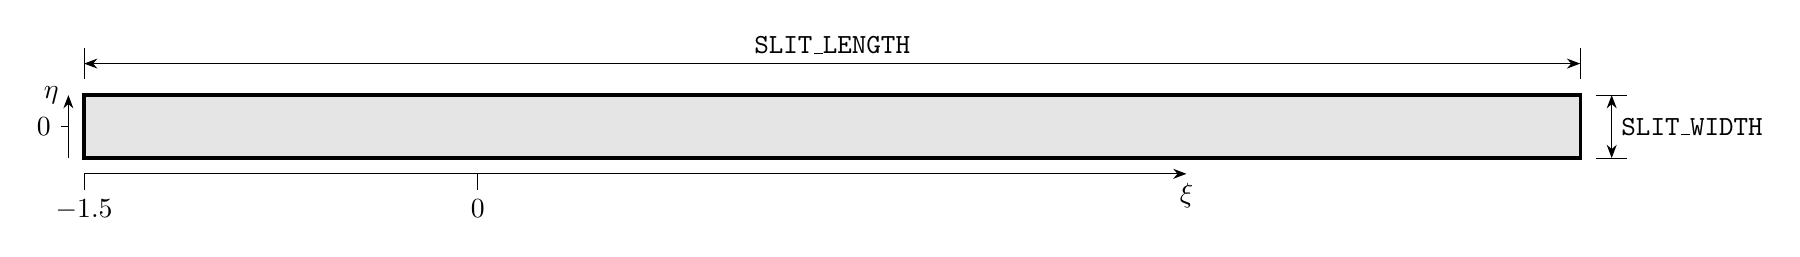
\begin{tikzpicture}[x=2cm, y=2cm]
%  \useasboundingbox({-2, -2}) rectangle ({5, 2});

  \draw [very thick, fill=gray!20](-1.5, -0.2) rectangle (8, 0.2);

  \draw (-1.5, 0.5) -- (-1.5, 0.3);
  \draw (8, 0.5) -- (8, 0.3);
  \draw [<->,>=Stealth] (-1.5, 0.4) -- (8, 0.4) node[midway,above]{\texttt{SLIT\_LENGTH}};

  \draw (8.1, 0.2) -- (8.3, 0.2);
  \draw (8.1, -0.2) -- (8.3, -0.2);
  \draw [<->,>=Stealth] (8.2, -0.2) -- (8.2, 0.2) node[midway,right]{\texttt{SLIT\_WIDTH}};

  \draw [->,>=Stealth] (-1.5, -0.3) -- (5.5, -0.3) node[below] {$\xi$};
  \draw (-1.5, -0.3) -- (-1.5, -0.4) node [below]{$-1.5$};
  \draw (1, -0.3) -- (1, -0.4) node [below]{$0$};

  \draw [->,>=Stealth] (-1.6, -0.2) -- (-1.6, 0.2) node [left]{$\eta$};
  \draw (-1.6, 0) -- (-1.65, 0) node [left]{$0$};
\end{tikzpicture}
\end{document}
